
%%%%%%%%%%%%%%%%%%%%%%%%%%%%%%%%%%%%%%%%%%%%%%%%%%%%%%%%%%%%%%%%%%%%%%%%
\chapter{Semantics of the \namee Calculus}
\label{chap:nested}
%%%%%%%%%%%%%%%%%%%%%%%%%%%%%%%%%%%%%%%%%%%%%%%%%%%%%%%%%%%%%%%%%%%%%%%%

This chapter presents \namee, a calculus based on \oname~\citep{oliveira2016disjoint} with disjoint intersection types that
features both BCD-style subtyping and the merge operator, which we believe
capture the essence of nested composition. We illustrate this by presenting a
solution to the expression problem based on family polymorphism. We then discuss
the algorithmic aspects of \namee. The coherence property of \namee is discussed
in \cref{chap:coherence:simple}.

\section{Overview}

\namee is a simple calculus with records and disjoint intersection types that
supports \emph{nested composition}. Nested composition enables encoding simple
forms of family polymorphism. More complex forms of family polymorphism,
involving binary methods~\citep{bruce1995binary} and mutable state are not yet
supported, but are interesting avenues for future work. Nevertheless, in \namee,
it is possible, for example, to encode \citeauthor{Ernst_2001}'s elegant family-polymorphism
solution to the expression problem. Compared to \oname the essential novelty of
\namee are distributivity rules between function/record types and intersection
types. These rules are the delta that enable extending the simple forms of
multiple inheritance/composition supported by \oname into a more powerful form
supporting nested composition. The distributivity rule between function types
and intersections is common in calculi with intersection types aimed at
capturing the set of all strongly normalizable terms, and was first proposed by
\citet{Barendregt_1983} (BCD). However the distributivity rule is not common in
calculi or languages with intersection types aimed at programming. For example
the rules employed in languages that support intersection types (such as Scala,
TypeScript, Flow or Ceylon) lack distributivity rules. Moreover distributivity
is also missing from several calculi with a merge operator. This includes all
calculi with disjoint intersection types~\citep{oliveira2016disjoint, alpuimdisjoint}
and \citeauthor{dunfield2014elaborating}'s work on elaborating
intersection types~\citep{dunfield2014elaborating}, which was the original
foundation for \oname. A possible reason for this omission in the past is that
distributivity adds substantial complexity (both algorithmically and
meta-theoretically), without having any obvious practical applications. This
chapter shows how to deal with the complications of BCD subtyping, while
identifying a major reason to include it in a programming language: BCD enables
nested composition and subtyping, which is of significant practical interest.

%The distributivity rules for records are
%new. Moreover, as far as we know, no previous work
%establishes the relation between BCD-style subtyping and nested composition.

\namee differs significantly from previous BCD-based calculi in that it has to
deal with the possibility of incoherence, introduced by the merge operator. Incoherence
is a non-issue in the previous BCD-based calculi because they do not feature
this merge operator or any other source of incoherence.
Although previous work on disjoint intersection types
proposes a solution to coherence, the solution imposes several ad-hoc restrictions (cf. \cref{sec:comparision})
to guarantee the uniqueness of the elaboration and thus allow for a simple
syntactic proof of coherence. Most
importantly, it makes it hard or impossible to adapt the proof to extensions of
the calculus, such as the new subtyping rules required by the BCD system.

In \namee we remove the brittleness of the previous syntactic method to prove
coherence, by employing a more semantic proof method based on \emph{logical
  relations}~\citep{tait, plotkin1973lambda, statman1985logical}. This new proof method has several
advantages. Firstly, with the new proof method, several restrictions that were
enforced by \oname to enable the syntactic proof are removed. For example
the work on \oname has to carefully distinguish between \emph{top-like types} and other types.
%This is necessary because top-like types can be
%non-disjoint (unlike other types), and yet they need to be allowed in a calculus
%with top types.
In \namee this distinction is not necessary; top-like types are handled like all
other types. Secondly, the new proof method is more powerful because it is based
on observational equivalence rather than syntactic equality; it is more robust
when the type system is extended. Finally, the removal of the ad-hoc
side-conditions makes adding new extensions, such as support for BCD-style
subtyping, easier. We shall return to this point in
\cref{chap:coherence:simple}.



\section{\namee by Examples}
\label{nested:sec:overview}

This section illustrates \namee with an encoding of a family polymorphism
solution to the expression problem, and informally presents its salient
features.


%-------------------------------------------------------------------------------
\subsection{The Expression Problem, \namee Style}

The \namee calculus allows us to solve the expression problem in a way that is
very similar to \citeauthor{Ernst_2001}'s \textsf{gbeta} solution in \cref{sec:ernst}.
However, the underlying mechanisms of \namee are quite different from those of
\textsf{gbeta}. In particular, \namee features a structural type system in which we can
model objects with records, and object types with record types. For instance, we
model the interface of \lstinline{Lang.Exp} with the singleton record type
\lstinline${ print : String }$. For the sake of conciseness, we use \lstinline{type} aliases
to abbreviate types.
\lstinputlisting[linerange=4-4]{./examples/overview.sl}% APPLY:linerange=PRINT_INTERFACE
Similarly, we capture the interface of the \lstinline{Lang} family in a record,
with one field for each case's constructor.
\lstinputlisting[linerange=8-8]{./examples/overview.sl}% APPLY:linerange=LANG_FAMILY
Here is the implementation of \lstinline{Lang}.
\lstinputlisting[linerange=17-24]{./examples/overview.sl}% APPLY:linerange=LANG_IMPL
We assume several primitive types: fixed width integers \lstinline{Int},
\lstinline{Double} for numeric operations and \lstinline{String} for text
manipulation. A \namee program consists of a collection of definitions and
declarations, separated by semicolon \lstinline{;}.

% - - - - - - - - - - - - - - - - - - - - - - - - - - - - - - - - - - - - - - - -
\paragraph{Adding evaluation.}
We obtain \lstinline{IPrint & IEval}, which is the corresponding type for \lstinline{LangEval.Exp}, by
intersecting \lstinline{IPrint} with \lstinline{IEval} where
\lstinputlisting[linerange=29-29]{./examples/overview.sl}% APPLY:linerange=EVAL_INTERFACE
The type for \lstinline{LangEval} is then
\lstinputlisting[linerange=34-37]{./examples/overview.sl}% APPLY:linerange=EVAL_PRINT_INTERFACE
We obtain an implementation for \lstinline{LangEval} by merging the existing
\lstinline{Lang} implementation \lstinline{implLang} with the new evaluation
functionality \lstinline{implEval} using the merge operator \lstinline{,,}.
\lstinputlisting[linerange=45-53]{./examples/overview.sl}% APPLY:linerange=EVAL_PRINT_IMPL

% - - - - - - - - - - - - - - - - - - - - - - - - - - - - - - - - - - - - - - - -
\paragraph{Adding negation.}
Adding negation to \lstinline{Lang} works similarly.
\lstinputlisting[linerange=57-65]{./examples/overview.sl}% APPLY:linerange=LANG_NEG
% \begin{Verbatim}[xleftmargin=10mm,fontsize=\relscale{.80}]
% type LangNeg = Lang & { neg : IPrint -> IPrint }

% implLangNeg : LangNeg
% implLangNeg = implLang ,, implNeg

% implNeg = { neg = \a.{print = "-" ++ a.print } }
% \end{Verbatim}

% - - - - - - - - - - - - - - - - - - - - - - - - - - - - - - - - - - - - - - - -
\paragraph{Putting everything together.}
Finally, we can combine the two extensions and provide the missing
implementation of evaluation for the negation case.
\lstinputlisting[linerange=70-80]{./examples/overview.sl}% APPLY:linerange=LANG_FINAL
We can test \lstinline{implLangNegEval} by creating an object that represents $-2 + 3$, which is able to print and evaluate at the same time.
\lstinputlisting[linerange=98-100]{./examples/overview.sl}% APPLY:linerange=TEST



%- - - - - - - - - - - - - - - - - - - - - - - - - - - - - - - - - - - - - - - -
\paragraph{Multi-field records.}
Recall that in \cref{bg:sec:intersection}, we show how to model multi-field records by
single-field records. Thus \namee does not have multi-field record types built in.
They are merely syntactic sugar for intersections of single-field record types.
Hence, the following is an equivalent definition of \lstinline{Lang}:
\lstinputlisting[linerange=13-13]{./examples/overview.sl}% APPLY:linerange=LANG_FAMILY2
Similarly, the multi-field record expression in the definition of
\lstinline{implLang} is syntactic sugar for the explicit merge of two
single-field records.
\begin{lstlisting}
implLang : Lang = { lit = ... } ,, { add = ... };
\end{lstlisting}

%- - - - - - - - - - - - - - - - - - - - - - - - - - - - - - - - - - - - - - - -
\paragraph{Subtyping.}
A distinctive difference compared to \textsf{gbeta} is that many more \namee types are related through
subtyping. Indeed, \textsf{gbeta} is unnecessarily conservative~\citep{ernst_hoh}: none of the families is related
through subtyping, nor is any of the class members of one family related to any
of the class members in another family. For instance, \lstinline{LangEval} is
not a subtype of \lstinline{Lang}, nor is \lstinline{LangNeg.Lit} a subtype
of \lstinline{Lang.Lit}.

In contrast, subtyping in \namee is much more nuanced and depends entirely on the
structure of types. The primary source of subtyping are intersection types:
any intersection type is a subtype of its components. For instance, 
\lstinline{IPrint & IEval} is a subtype of both \lstinline{IPrint} and
\lstinline{IEval}. Similarly \lstinline{LangNeg = Lang & NegPrint} is a subtype
of \lstinline{Lang}. Compare this to \textsf{gbeta} where \lstinline{LangEval.Expr} is
not a subtype of \lstinline{Lang.Expr}, nor is the family \lstinline{LangNeg} a
subtype of the family \lstinline{Lang}.

However, \textsf{gbeta} and \namee agree that \lstinline{LangEval} is not a subtype of
\lstinline{Lang}. The \namee-side of this may seem contradictory at first, as we
have seen that intersection types arise from the use of the merge operator.
We have created an implementation for \lstinline{LangEval} with
\lstinline{implLang ,, implEval} where \lstinline{implLang} has type \lstinline{Lang}, which
suggests that \lstinline{LangEval} is a subtype of \lstinline{Lang}.
Yet, there is a flaw in our reasoning:
strictly speaking, \lstinline{implLang ,, implEval} is not of
type \lstinline{LangEval} but instead of type \lstinline{Lang & EvalExt}, where
\lstinline{EvalExt} is the type of \lstinline{implEval}:
\lstinputlisting[linerange=41-41]{./examples/overview.sl}% APPLY:linerange=EVAL_INTERFACE2

Nevertheless, the definition of \lstinline{implLangEval} is valid because
\lstinline{Lang & EvalExt} is a subtype of \lstinline{LangEval}.
Indeed, if we consider for the sake of simplicity only the \lstinline{lit}
field, we have that \lstinline{(Int -> IPrint) & (Int -> IEval)} is a
subtype of \lstinline{Int -> IPrint & IEval}. This follows from a standard
subtyping axiom for distributivity of functions and intersections in the BCD system inherited by \namee.
In conclusion, \lstinline{Lang & EvalExt} is a subtype of both \lstinline{Lang}
and of \lstinline{LangEval}. However, neither of the latter two types is a subtype of the other.
Indeed, \lstinline{LangEval} is not a subtype of \lstinline{Lang} as the type
of \lstinline{add} is not covariantly refined and thus admitting the subtyping
is unsound. For the same reason \lstinline{Lang} is not a subtype of \lstinline{LangEval}.


A summary of the various relationships between the language components is shown
in \cref{fig:diagram}. Admittedly, the figure looks quite complex because our
calculus has a structural type system (as often more foundational calculi
do) where more types are related through subtyping, whereas mainstream object-oriented
languages have nominal type systems.



\begin{figure}[t]
  \centering
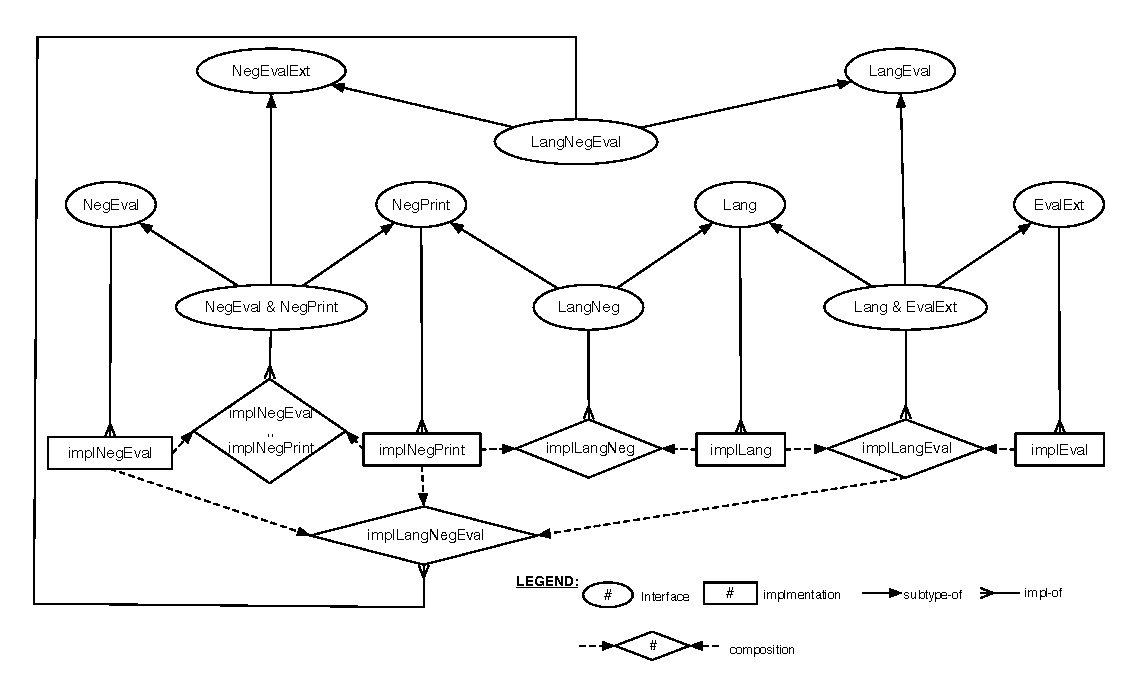
\includegraphics[scale=0.75]{figures/diagram.eps}
\caption{Summary of the relationships between language components}
\label{fig:diagram}
\end{figure}


\paragraph{Stand-alone extensions.}
Unlike in \textsf{gbeta} and other class-based inheritance systems, in \namee
the extension \lstinline{implEval} is not tied to \lstinline{LangEval}. In that
sense, it resembles trait and mixin systems that can apply the same extension
to different classes. However, unlike those systems, \lstinline{implEval} can also
exist as a value on its own, i.e., it is not an extension per se.

%-------------------------------------------------------------------------------
% \subsection{Disjoint Intersection Types and Ambiguity}

% The above example shows that intersection types and the merge operator
% are closely related to multiple
% inheritance. Indeed, they share a major concern with multiple inheritance,
% namely ambiguity. When a subclass inherits an implementation of the same
% method from two different parent classes, it is unclear which of the two
% methods is to be adopted by the subclass. In the case where the two parent classes
% have a common superclass, this is known as the \emph{diamond problem}.
% The ambiguity problem also appears in \namee,
% e.g., if we merge two numbers to obtain $\mer{1}{2}$ of type
% $\inter{\mathsf{Int}}{\mathsf{Int}}$. Is the result of $\mer{1}{2} + 3$
% either $4$ or $5$?

% Disjoint intersection types offer to statically detect potential ambiguity and
% to ask the programmer to explicitly resolve the ambiguity by rejecting the
% program in its ambiguous form. In the previous work on \oname, ambiguity is
% avoided by dictating that all intersection types have to be disjoint, i.e.,
% $\inter{\mathsf{Int}}{\mathsf{Int}}$ is ill-formed because the first component
% has the same type as the second.


% Disjoint intersection types ensure unambiguity and conflicts are
% statically detected and manually resolved by programmers. This
% is similar to the trait model.


% Local Variables:
% TeX-master: "../../Thesis"
% org-ref-default-bibliography: ../../Thesis.bib
% End:


\newcommand{\rulehl}[2][gray!40]{%
  \colorbox{#1}{$\displaystyle#2$}}

\section{Syntax and Semantics}
\label{sec:typesystem}

In this section we formally present the syntax and semantics of \namee. Compared
to prior work~\cite{alpuimdisjoint, oliveira2016disjoint}, \namee has a more
powerful subtyping relation. The new subtyping relation is inspired by BCD-style
subtyping, but with two noteworthy differences: subtyping is coercive (in
contrast to traditional formulations of BCD); and it is extended with records.
We also have a new target language with explicit coercions inspired by the coercion calculus of
Henglein~\cite{Henglein_1994}. A full technical comparison between \namee and \oname can be found in \cref{sec:comparision}.


\subsection{Syntax}

\Cref{fig:source} shows the syntax of \namee.
% with the differences from \oname \hll{highlighted}.
% \namee is a simple calculus with intersection types, the merge operator
% and singleton records.
For brevity of the meta-theoretic study, we do not
consider primitive operations on integers, or other primitive types.
They can be easily added to the language, and our prototype implementation is
indeed equipped with common primitive types and their operations.
Metavariables $[[A]], [[B]], [[C]]$ range over types. Types include the type of integers
$[[nat]]$, a top type $[[Top]]$, function types $[[A -> B]]$, intersection types
$[[A & B]]$, and singleton record types $[[ {l : A} ]]$. Metavariable $[[ee]]$
ranges over expressions. Expressions include variables $[[x]]$, integers $[[i]]$,
a canonical top value $[[Top]]$, lambda abstractions $[[\x . ee]]$,
applications $[[ee1 ee2]]$, merges $[[ee1 ,, ee2]]$, annotated terms $[[ee : A]]$,
singleton records $[[ {l = ee}]]$, and record selections $[[ee.l ]]$.

\begin{figure}[t]
  \centering
\begin{tabular}{llll}\toprule
  Types & $[[A]], [[B]], [[C]]$ & $\Coloneqq$ & $[[nat]] \mid [[Top]] \mid [[A -> B]]  \mid [[A & B]] \mid [[ { l : A } ]]$ \\
  Expressions & $[[ee]]$ & $\Coloneqq$ & $[[x]] \mid [[i]] \mid [[Top]] \mid [[\x . ee]] \mid [[ee1 ee2]] \mid [[ee1 ,, ee2]] \mid [[ee : A]]  $ \\
  & & $\mid$ & $ [[ { l = ee } ]] \mid [[ee.l]] $ \\
  Typing contexts & $[[GG]]$ & $\Coloneqq$ & $[[empty]] \mid [[GG , x : A]]$ \\ \bottomrule
\end{tabular}
  \caption{Syntax of \namee}
  \label{fig:source}
\end{figure}

\subsection{Declarative Subtyping}

\Cref{fig:subtype_decl} presents the subtyping relation. We ignore the
\hll{highlighted} parts, and explain them later in \cref{sec:elaboration}.

\begin{figure}[t]
  \centering
  \drules[S]{$[[A <: B ~~> c]]$}{Declarative subtyping}{refl, trans, top, rcd, arr, andl, andr, and, distArr, topArr, distRcd, topRcd}
  \caption{Declarative specification of subtyping}
  \label{fig:subtype_decl}
\end{figure}

\paragraph{BCD-Style Subtyping.}
The subtyping rules are essentially those of the BCD type
system~\cite{Barendregt_1983}, extended with subtyping for singleton records.
\Rref{S-top,S-rcd} for top types and record types are straightforward.
\Rref{S-arr} for function subtyping is standard. \Rref{S-andl,S-andr,S-and} for
intersection types axiomatize that $[[A & B]]$ is the greatest lower bound of
$[[A]]$ and $[[B]]$. \Rref{S-distArr} is perhaps the most interesting rule.
This, so-called ``distributivity'' rule, describes the interaction between
the subtyping relations for function types and those for intersection types.
Note that the other direction $[[A1 -> A2 & A3 <: (A1 -> A2) & (A1 -> A3)]]$
and the contravariant distribution $[[ (A1 -> A2) & (A3 -> A2) <: A1 & A3 -> A2 ]]$ are both
derivable from the existing subtyping rules, as shown below:
  \begin{footnotesize}
\begin{mathpar}
  \inferrule*[right=\rref*{S-and}]
  {  \inferrule*[right=\rref*{S-arr}]{ [[ A1 <: A1  ]] \\ [[ A2 & A3 <: A2  ]]  }{[[   A1 -> A2 & A3 <: A1 -> A2  ]]} \\
    \inferrule*[right=\rref*{S-arr}]{ [[ A1 <: A1  ]] \\ [[ A2 & A3 <: A3  ]] }{[[ A1 -> A2 & A3 -> A1 -> A3      ]]}  }
  {  [[ A1 -> A2 & A3 <: (A1 -> A2) & (A1 -> A3)  ]]  }
\end{mathpar}
\begin{mathpar}
  \inferrule*[right=\rref*{S-trans}]
  {  \inferrule*[right=\rref*{S-andl}]{ }{[[ (A1 -> A2) & (A3 -> A2) <: A1 -> A2   ]]} \\
    \inferrule*[right=\rref*{S-arr}]{ [[ A1 & A3 <: A1  ]] \\ [[ A2 <: A2  ]] }{[[ A1 -> A2 <: A1 & A3 -> A2  ]]}  }
  {  [[  (A1 -> A2) & (A3 -> A2) <: A1 & A3 -> A2  ]]   }
\end{mathpar}
  \end{footnotesize}
\Rref{S-distRcd}, which is not found in the original BCD system,
prescribes the distribution of records over intersection types. The two
distributivity rules are the key to enable nested composition. The rule
\rref*{S-topArr} is standard in BCD subtyping, and the new
\rref{S-topRcd} plays a similar role for record types.

\paragraph{Non-Algorithmic.}
The subtyping relation in \cref{fig:subtype_decl} is clearly no more than a
specification due to the two subtyping axioms: \rref{S-refl,S-trans}. A sound
and complete algorithmic version is discussed in \cref{sec:alg}. Nevertheless,
for the sake of establishing coherence, the declarative subtyping relation is
sufficient.


\paragraph{Property of Subtyping.}
The subtyping relation is vacuously \textit{reflexive} and \textit{transitive}.



\subsection{Typing of \namee}


\begin{figure}[t]
  \centering
\drules[T]{$[[GG  |- ee => A ~~> e]]$}{Inference}{top, lit, var, app, anno, proj, merge, rcd}
\drules[T]{$[[GG  |- ee <= A ~~> e]]$}{Checking}{abs, sub}
  \caption{Bidirectional type system of \namee}
  \label{fig:type_system}
\end{figure}

% no gray anymore after this point
\renewcommand{\rulehl}[1]{#1}



The bidirectional type system for \namee is shown in \cref{fig:type_system}.
Again we ignore the \hll{highlighted} parts for now.

% The main difference to \oname is the absence of a well-formedness
% judgement. Unlike \oname, which requires a well-formedness judgement to ensure
% that all intersection types are disjoint, \namee only requires a disjointness
% check at the merge operator. Non-disjoint types such as $[[nat & nat]]$ are
% allowed in other parts of the program.

\begin{comment}
Unlike the development of \oname, which first presents a type assignment
specification, \Cref{fig:type_system} directly present the bidirectional type
system of \namee.
Unfortunately, we found that their declarative type
system is incoherent in nature (even with all the syntactic restrictions).
\jeremy{perhaps add a counter example somewhere?} Again, the reader is advised
to continue ignoring the gray-shaded parts until \cref{sec:elaboration}.
\tom{The above story is a bit confusing to me. Is it the case that the
     \oname paper already was aware of the coherence problem with its
     declarative type system and for that reason (and inference) presented
     a bidirection type system as well? If so, that's not clear.} \jeremy{I
     remember at one point Bruno and I believed the declarative system is
     coherent, it's just hard to prove. Then I found a counterexample. That was
     after \tname paper.  }
\end{comment}


\begin{figure}[t]
  \centering
  \drules[D]{$[[A ** B]]$}{Disjointness}{topL, topR, arr, andL, andR, rcdEq, rcdNeq,ax}
  \drules[Dax]{$[[A **a B]]$}{Disjointness axioms}{sym, intArr, intRcd,arrRcd}
  \caption{Disjointness}
  \label{fig:disjoint}
\end{figure}


\paragraph{Typing Rules and Disjointness.}

As with traditional bidirectional type systems, we employ two modes: the
inference mode ($[[=>]]$) and the checking mode ($[[<=]]$). The inference
judgement $[[GG |- ee => A]]$ says that we can synthesize a type $[[A]]$ for
expression $[[ee]]$ in the context $[[GG]]$. The checking judgement $[[GG |- ee
<= A]]$ checks $[[ee]]$ against $[[A]]$ in the context $[[GG]]$. The
disjointness judgement $[[A ** B]]$ used in \rref{T-merge} is shown in
\cref{fig:disjoint}, which states that the types $[[A]]$ and $[[B]]$ are
\textit{disjoint}. The intuition of two types being disjoint is
that their least upper bound is (isomorphic to) $[[Top]]$. The disjointness judgement is
important in order to rule out ambiguous expressions such as $\mer{1}{2}$. Most
of the typing and disjointness rules are standard and are explained in detail in
previous work~\cite{oliveira2016disjoint, alpuimdisjoint}.
%We refer
%the reader to their papers for further explanation.


\subsection{Elaboration Semantics}
\label{sec:elaboration}

\begin{figure}[t]
  \centering
\begin{tabular}{llll} \toprule
  Types & $[[T]]$ & $\Coloneqq$ & $[[nat]] \mid [[Unit]] \mid [[T1 * T2]] \mid [[T1 -> T2]] $ \\
  Terms & $[[e]]$ & $\Coloneqq$ & $[[x]] \mid [[i]] \mid [[unit]] \mid [[\x . e]] \mid [[e1 e2]] \mid [[<e1, e2>]] \mid [[c e]]$ \\
  Coercions & $[[c]]$ & $\Coloneqq$ & $ [[id]] \mid [[c1 o c2]] \mid [[top]] \mid [[c1 -> c2]] \mid [[<c1, c2>]] \mid [[pp1]] \mid [[pp2]] $ \\
  &  &  $\mid$ & $   [[distArr]] \mid [[topArr]]  $ \\
  Values & $[[v]]$ & $\Coloneqq$ & $[[unit]] \mid [[i]] \mid [[\x.e]] \mid  [[<v1, v2>]] \mid [[(c1 -> c2) v]] \mid [[distArr v]] \mid [[topArr v]] $ \\
  Typing contexts & $[[gg]]$ & $\Coloneqq$ & $[[empty]] \mid [[gg , x : T]]$ \\
  Evaluation Contexts & $[[EE]]$ & $\Coloneqq$ &  $  [[__]] \mid [[EE e]] \mid [[v EE]] \mid [[ < EE , e >  ]] \mid [[ < v , EE > ]] \mid [[ c EE  ]]$ \\ \bottomrule
\end{tabular}
  \caption{\tname syntax}
  \label{fig:target}
\end{figure}

The operational semantics of \namee is given by elaborating source expressions
$[[ee]]$ into target terms $[[e]]$. Our target language \tname is the standard
simply-typed call-by-value $\lambda$-calculus extended with products and coercions.
The syntax of \tname is shown in \cref{fig:target}. The
meta-function $| \cdot |$ shown in \cref{def:type:translate} transforms \namee
types to \tname types, and extends naturally to typing contexts.

\begin{definition}[Type translation from \namee to \tname] \label{def:type:translate}
  \begin{align*}
    | [[nat]] | &= [[nat]] \\
    | [[Top]] | &= \langle \rangle \\
    | [[A -> B]]  | &= [[ | A | -> | B |  ]] \\
    | [[ A & B  ]] | &= [[ | A | * | B |  ]] \\
    | \recordType{l}{A} | &= | A |
  \end{align*}
\end{definition}



\paragraph{Explicit Coercions and Coercive Subtyping.}

The separate syntactic category for explicit coercions is a distinct
difference from the prior works (in which they are regular terms). Our coercions
are based on those of Henglein~\cite{Henglein_1994}, and we add more forms due to our
extra subtyping rules.
Metavariable $[[c]]$ ranges over coercions.\footnote{Coercions $[[pp1]]$ and $[[pp2]]$ subsume the first and second projection of pairs, respectively.}
Coercions express the conversion
of a term from one type to another. Because of the addition of coercions, the
grammar contains explicit coercion applications $[[c e]]$ as a term, and various
unsaturated coercion applications as values. The use of explicit coercions is useful for the new semantic
proof of coherence based on logical relations.
The subtyping judgement in \cref{fig:subtype_decl} has the form $[[A <: B ~~> c]]$, which says that the
subtyping derivation of $[[A <: B]]$ produces a coercion $[[c]]$ that converts
terms of type $[[ |A| ]]$ to type $[[ |B| ]]$. Each subtyping rule has its own
specific form of coercion.

%The meaning of the different forms of coercions becomes clear in \tom{Section
%  TODO} \jeremy{it's a paragraph, how to refer it?} which explains coercive
%subtyping.\bruno{Why not discuss the form of coercions directly here?}


\paragraph{Target Typing.}
The typing of \tname has the form $[[gg |- e : T]]$, which is entirely standard. Only the typing of coercion
applications, shown below, deserves attention:
\begin{mathpar}
\drule{t-capp}
\end{mathpar}
Here the judgement $[[c |- T1 tri T2]]$ expresses the typing of coercions, which
are essentially functions from $[[T1]]$ to $[[T2]]$. Their typing
rules correspond exactly to the subtyping rules of \namee, as
shown in \cref{fig:co}.

\begin{figure}[t]
  \centering
  \drules[ct]{$[[c |- T1 tri T2]]$}{Coercion typing}{refl, trans, top, topArr, arr, pair, projl, projr, distArr}
  \caption{Coercion typing}
  \label{fig:co}
\end{figure}

\paragraph{Dynamic Semantics.}

\begin{figure}[t]
  \centering
\drules[r]{$[[e --> e']]$}{Single-step reduction}{id, trans, top, topArr, pair, arr, distArr, projl, projr, app, ctxt}
  \caption{Dynamic semantics of \tname}
  \label{fig:coercion_red}
\end{figure}

The dynamic semantics of \tname is shown in \cref{fig:coercion_red}. We write
$[[e --> e']]$ for reduction of expressions. The first three lines are reduction
rules for coercions. They do not contribute to computation but merely rearrange
coercions. Our coercion reduction rules are quite standard but not efficient in
terms of space. Nevertheless, there is existing work on space-efficient
coercions~\cite{Siek_2015, herman2010space}, which should be applicable to our
work as well. \Rref{r-app} is the usual $\beta$-rule that performs actual
computation, and \rref{r-ctxt} handles reduction under an evaluation context. As
standard, $[[-->>]]$ is the reflexive, transitive closure of $[[-->]]$.
Now we can show that \tname is type safe:
\begin{theorem}[Preservation]
  If $[[empty |- e : T]]$ and $[[e --> e']]$, then $[[empty |- e' : T]]$.
\end{theorem}
\begin{theorem}[Progress]
  If $[[empty |- e : T]]$, then either $[[e]]$ is a value, or there exists $[[e']]$ such
  that $[[e --> e']]$.
\end{theorem}




\paragraph{Elaboration.}
\begin{comment}
The subtyping judgement in \cref{fig:subtype_decl} has the form $[[A <: B ~~> c]]$, which says that the subtyping
derivation of $[[A <: B]]$ produces a coercion $[[c]]$ that is used to convert a
term of type $[[ |A| ]]$ to type $[[ |B| ]]$. Each
subtyping rule has its own specific form of coercion.
\end{comment}
We are now in a position to explain the elaboration judgements $[[GG |- ee
=> A ~~> e]]$ and $[[GG |- ee <= A ~~> e]]$ in \cref{fig:type_system}. The only
interesting rule is \rref{T-sub}, which applies the coercion $[[c]]$ produced by
subtyping to the target term $[[e]]$ to form a coercion application
$[[c e]]$. All the other rules do straightforward translations between
source and target expressions.


To conclude, we show two lemmas that relate \namee expressions
to \tname terms.
% (Note that in this and subsequent sections, we only provide
% a proof sketch for each lemma and theorem. We refer the interested reader
% to our Coq development for the full proofs.)

\begin{lemma}[Coercions preserve types]
  If $[[A <: B ~~> c]]$, then $[[c |-  |A| tri |B|]]$.
  \label{lemma:sub-correct}
\end{lemma}
\begin{proof}
  By structural induction on the derivation of subtyping.
\end{proof}


\begin{lemma}[Elaboration soundness] We have that:
  \begin{itemize}
  \item If $[[GG |- ee => A ~~> e]]$, then $|\Gamma| \vdash e : |A| $.
  \item If $[[GG |- ee <= A ~~> e]]$, then $|\Gamma| \vdash e : |A| $.
  \end{itemize}
\end{lemma}
\begin{proof}
  By structural induction on the derivation of typing.
\end{proof}

\subsection{Comparison with \oname}
\label{sec:comparision}

Below we identify major differences between \namee and \oname, which, when
taken together, yield a simpler and more elegant system. The differences may seem
superficial, but they have far-reaching impacts on the semantics, especially on
coherence, our major topic in \cref{chap:coherence:simple}.

\paragraph{No Ordinary Types.}

Apart from the extra subtyping rules, there is an important difference from the
\oname subtyping relation. The subtyping relation of \oname employs an
auxiliary unary relation called $\mathsf{ordinary}$, which plays a fundamental
role for ensuring coherence and obtaining an
algorithm~\cite{Davies_2000}. The \namee calculus discards the notion of
ordinary types completely; this yields a clean and elegant formulation of the
subtyping relation. Another minor difference is that due to the addition of the
transitivity axiom (\rref{S-trans}), \rref{S-andl,S-andr} are simplified: an
intersection type $[[A & B]]$ is a subtype of both $[[A]]$ and $[[B]]$, instead
of the more general form $[[ A & B <: C]]$.

% \paragraph{Example}
% The following example shows the derivation tree of the subtyping example
% presented in \cref{sec:overview}. \jeremy{A derivation of the nested composition
%   example? }


\paragraph{No Top-Like Types.}

There is a notable difference from the coercive subtyping of \oname. Because of
their syntactic proof method, they have special treatment for coercions of
\textit{top-like types} in order to retain coherence. For \namee, as
with ordinary types, we do not need this kind of ad-hoc treatment, thanks to the
adoption of a more powerful proof method (cf. \cref{chap:coherence:simple}).




\paragraph{No Well-Formedness Judgement.}

A key difference from the type system of \oname is the complete omission of the
well-formedness judgement. In \oname, the well-formedness judgement $[[GG |- A]]$
appears in both \rref{T-abs,T-sub}. The sole purpose of this judgement is
to enforce the invariant that all intersection types are disjoint. However, as
\cref{chap:coherence:simple} will explain, the syntactic restriction is unnecessary for
coherence, and merely complicates the type system. The \namee calculus discards
this well-formedness judgement altogether in favour of a simpler design that is
still coherent. An important implication is that even without adding BCD subtyping,
\namee is already more expressive than \oname: an expression such as $1 : [[nat & nat]]$ is accepted in
\namee but rejected in \oname. This simplification is based on an important
observation: incoherence can only originate in merges. Therefore disjointness
checking is only necessary in \rref{T-merge}.


% Local Variables:
% TeX-master: "../../Thesis"
% org-ref-default-bibliography: ../../Thesis.bib
% End:


\section{Algorithmic Subtyping}
\label{sec:alg}

This section presents an algorithm that implements the subtyping relation in
\cref{fig:subtype_decl}. While BCD subtyping is well-known, the
presence of a transitivity axiom in the rules means that the system is
not algorithmic. This raises an obvious question: how to obtain an
algorithm for this subtyping relation? Laurent~\cite{Laurent12note} has shown that simply dropping
the transitivity rule from the BCD system is not possible without losing expressivity. Hence, this avenue for
obtaining an algorithm is not available. 
%Moreover, even if transitivity elimination
%would be possible, the remaining rules are still highly overlapping, and pose
%difficulties for an implementation.  
Instead, we adapt Pierce's decision
procedure~\cite{pierce1989decision} for a subtyping system (closely
related to BCD) to obtain a sound and complete algorithm for our
BCD extension. Our algorithm extends Pierce's decision
procedure with subtyping of singleton records and
coercion generation. We prove in Coq that the algorithm is sound and complete with
respect to the declarative version. At the same time we
find some errors and missing lemmas in Pierce's original manual proofs.

%The algorithm is implemented in our
%prototype implementation. \jeremy{should i say more about implementation?}

%See \cref{sec:alg} for the details. 
%\bruno{The meaning of the paragraph is somewhat obscure to me. After
%  discussing with Tom, it seems that what may be meant here is that we
%cannot do cut elimination, which is a common process that you can try
%for certain systems with subtyping. However Pierce managed to find
%another way to get a sound/complete algorithmic system. Maybe 
%the text can be improved.}


\subsection{The Subtyping Algorithm}

\begin{figure}[t]
  \centering
  \begin{small}
  \drules[A]{$[[fs |- A <: B ~~> c]]$}{Algorithmic subtyping}{and, arr, rcd, top, arrNat, rcdNat, andNOne, andNTwo, nat}
  \end{small}
  \caption{Algorithmic subtyping of \name}
  \label{fig:algorithm}
\end{figure}


\Cref{fig:algorithm} shows the algorithmic subtyping judgement $[[fs |- A <: B ~~> c]]$.
This judgement is the algorithmic counterpart of the declarative
judgement $[[A <: fs -> B ~~> c]]$, where the symbol $[[fs]]$ stands for a
queue of types and labels. Definition~\ref{def:fs} converts a queue to a type:
\begin{definition} $[[fs -> A]]$ is inductively defined as follows: \label{def:fs}
  \begin{mathpar}
    [[ [] -> A]] = [[A]] \and
    [[ (fs , B) -> A]] = [[fs -> (B -> A)]] \and
    [[ (fs , {l}) -> A]] = [[fs -> {l : A}]]
  \end{mathpar}
\end{definition}
For instance, if $[[fs]] = [[A]] , [[B]] , \{[[l]]\} $, then $[[fs -> C]]$ abbreviates $ [[A -> B -> {l : C}]]$.

The basic idea of $[[fs |- A <: B ~~> c]]$ is to first perform a structural
analysis of $[[B]]$, which descends into both sides of $[[&]]$'s (\rref{A-and}),
into the right side of $[[->]]$'s (\rref{A-arr}), and into the fields of records
(\rref{A-rcd}) until it reaches one of the two base cases, $[[nat]]$ or
$[[Top]]$. If the base case is $[[Top]]$, then the subtyping holds trivially
(\rref{A-top}). If the base case is $[[nat]]$, the algorithm performs a
structural analysis of $[[A]]$, in which $[[fs]]$ plays an important role. The
left sides of $[[->]]$'s are pushed onto $[[fs]]$ as they are encountered in
$[[B]]$ and popped off again later, left to right, as $[[->]]$'s are encountered
in $[[A]]$ (\rref{A-arrNat}). Similarly, the labels are pushed onto $[[fs]]$ as
they are encountered in $[[B]]$ and popped off again later, left to right, as
records are encountered in $[[A]]$ (\rref{A-rcdNat}). The remaining rules are
similar to their declarative counterparts. Let us illustrate the algorithm
with an example
derivation (for space reasons we use $[[N]]$ and $[[S]]$ to denote $[[nat]]$ and $[[string]]$ respectively),
which is essentially the one used by the \lstinline{add} field in \cref{sec:overview}. The
readers can try to give a corresponding derivation using the declarative
subtyping and see how \rref{S-trans} plays an essential role there.
\begin{small}
\begin{mathpar}
  \inferrule*[right=\rref*{A-rcd}]
  { \inferrule*[right=\rref*{A-arr}(\textit{twice})]
    { \inferrule*[right=\rref*{A-and}]
      { D \\ D' }
      { \{ [[l]]  \}, [[N & S]] ,[[N & S]] \vdash [[{l : N -> N -> N} & {l : S -> S -> S} ]] \prec : [[N & S]] }  }
    { \{ [[l]]  \} \vdash [[{l : N -> N -> N} & {l : S -> S -> S} ]] \prec : [[ N & S -> N & S -> N & S ]]}      }
  {  [[{l : N -> N -> N} & {l : S -> S -> S}]] \prec : [[{l : N & S -> N & S -> N & S}]]   }
\end{mathpar}
\end{small}
where the sub-derivation $D$ is shown below ($D'$ is similar):
\begin{small}
\begin{mathpar}
\inferrule*[right=\rref*{A-andN1}]
        { \inferrule*[right=\rref*{A-rcdNat}]
          { \inferrule*[right=\rref*{A-arrNat}]
            { \inferrule*{ \dots } { [[N & S]] \prec : [[N]] }
              \\
              \inferrule* {\dots} { [[N & S]] \vdash [[N -> N]] \prec : [[N]] }     }
            {[[N & S]] ,[[N & S]] \vdash [[N -> N -> N]] \prec : [[N]]} }
          { \{ [[l]]  \}, [[N & S]] ,[[N & S]] \vdash [[{l : N -> N -> N}]] \prec : [[N]] } }
        { \{ [[l]]  \}, [[N & S]] ,[[N & S]] \vdash [[{l : N -> N -> N} & {l : S -> S -> S} ]] \prec : [[N]] }
\end{mathpar}
\end{small}
Now consider the coercions. Algorithmic subtyping uses the same set of
coercions as declarative subtyping. However, because algorithmic
subtyping has a different structure, the rules generate slightly more
complicated coercions. Two meta-functions $\llbracket \cdot \rrbracket_{\top}$
and $\llbracket \cdot \rrbracket_{\&}$ used in \rref{A-top,A-and} respectively,
are meant to generate correct forms of coercions. They are defined recursively
on $[[fs]]$ and are shown in \cref{fig:coercion}.

\begin{figure}[t]
    \centering
    \begin{small}
    \begin{subfigure}[b]{0.5\textwidth}
      \begin{align*}
        [[ < [] >1 ]] &=  [[top]] \\
        [[ < { l } , fs >1 ]] &= [[ {l : < fs >1} o < l >  ]] \\
        [[ < A , fs >1 ]] &= [[(top -> < fs >1) o (topArr o top)]]
      \end{align*}
    \end{subfigure} ~
    \begin{subfigure}[b]{0.45\textwidth}
      \begin{align*}
        [[ < [] >2 ]] &=  [[id]] \\
        [[ < { l } , fs >2 ]] &= [[ {l : < fs >2} o distRcd l  ]] \\
        [[ < A , fs >2 ]] &= [[(id -> < fs >2) o distArr]]
      \end{align*}
    \end{subfigure}
    \end{small}
    \caption{Meta-functions of coercions}\label{fig:coercion}
\end{figure}

\subsection{Correctness of the Algorithm}

To establish the correctness of the algorithm, we must show that the algorithm
is both sound and complete with respect to the declarative specification. While
soundness follows quite easily, completeness is much harder. The proof of
completeness essentially follows that of Pierce~\cite{pierce1989decision}
%%\footnote{
%%While transferring \cite{pierce1989decision}'s manual proofs to Coq,
%%we discovered several errors, which will be reported along the way.}
in that we
need to show the algorithmic subtyping is reflexive and
transitive. 


\paragraph{Soundness of the Algorithm.}

The following two lemmas connect the declarative subtyping with the meta-functions.

\begin{lemma} \label{lemma:top}
  $[[ Top <: fs -> Top ~~> < fs >1]]$
\end{lemma}
\begin{proof}
  By induction on the length of $[[fs]]$.
\end{proof}

\begin{lemma} \label{lemma:and}
  $[[(fs -> A) & (fs -> B) <: fs -> (A & B) ~~> < fs >2]]$
\end{lemma}
\begin{proof}
  By induction on the length of $[[fs]]$.
\end{proof}

The proof of soundness is straightforward.
\begin{theorem}[Soundness] \label{thm:soundness}
  If $[[ fs |- A <: B ~~> c]]$ then $[[A]] <: [[fs]] \rightarrow [[B]] [[~~>]] [[c]]$.
\end{theorem}
\begin{proof}
  By induction on the derivation of the algorithmic subtyping and applying \cref{lemma:top,lemma:and} where appropriate.
\end{proof}


\paragraph{Completeness of the Algorithm.}


\newcommand{\UU}[1]{\mathcal{U}(#1)}

Completeness, however, is much harder. The reason is that, due to the use of
$[[fs]]$, reflexivity and transitivity are not entirely obvious. We need to
strengthen the induction hypothesis by introducing the notion of a set,
$\UU{[[A]]}$, of ``reflexive supertypes'' of $[[A]]$, as defined below:
\begin{mathpar}
  \UU{[[Top]]} \defeq \{ [[Top]]  \} \and
  \UU{[[nat]]} \defeq \{ [[nat]]  \} \and
  \UU{[[{l : A}]]} \defeq \{ [[{l : B}]] \mid [[B]] \in \UU{[[A]]}  \} \and
  \UU{[[A & B]]} \defeq \UU{[[A]]} \cup \UU{[[B]]} \cup \{ [[A & B]] \} \and
  \UU{[[A -> B]]} \defeq \{ [[A -> C]] \mid [[C]] \in \UU{[[B]]} \}
\end{mathpar}
We show two lemmas about $\UU{[[A]]}$ that are crucial in the subsequent proofs.
\begin{lemma} \label{lemma:set_refl}
  $[[A]] \in \UU{[[A]]}$
\end{lemma}
\begin{proof}
  By induction on the structure of $[[A]]$.
\end{proof}

\begin{lemma} \label{lemma:set_trans}
  If $[[A]] \in \UU{[[B]]}$ and $[[B]] \in \UU{[[C]]}$, then $[[A]] \in \UU{[[C]]}$.
\end{lemma}
\begin{proof}
  By induction on the structure of $[[B]]$.
\end{proof}

\begin{remark}
  Lemma~\ref{lemma:set_trans} is not found in Pierce's proofs~\cite{pierce1989decision}, which is
  crucial in Lemma~\ref{lemma:refl0}, from which reflexivity (Lemma~\ref{lemma:refl})
  follows immediately.
\end{remark}

% Next we show the following lemma from which reflexivity (Lemma~\ref{lemma:refl})

\begin{lemma} \label{lemma:refl0}
  If $[[fs -> B]] \in \UU{[[A]]}$ then there exists $[[c]]$ such that $[[fs |- A <: B ~~> c]]$.
\end{lemma}
\begin{proof}
  By induction on $\mathsf{size}([[A]]) + \mathsf{size}([[B]]) + \mathsf{size}([[fs]])$.
\end{proof}
% \begin{remark}
%   \cite{pierce1989decision}'s proof is wrong in one case~\cite[pp.~10, Case~ii]{pierce1989decision} because we need \cref{lemma:set_trans} to be able
%   to apply the inductive hypothesis.
% \end{remark}

Now it immediately follows that the algorithmic subtyping is reflexive.

\begin{lemma}[Reflexivity] \label{lemma:refl}
  For every $[[A]]$ there exists $[[c]]$ such that $[[ [] |- A <: A ~~> c]]$.
\end{lemma}
\begin{proof}
  Immediate from Lemma~\ref{lemma:set_refl} and Lemma~\ref{lemma:refl0}.
\end{proof}

We omit the details of the proof of transitivity.
%The proof of transitivity is, to quote \cite{pierce1989decision}, typically
%``the hardest single piece'' of metatheory. We omit the details here for lack of space and
%refer the interested reader to our Coq development.

\begin{lemma}[Transitivity] \label{lemma:trans}
  If $[[ [] |- A1 <: A2 ~~> c1]]$ and $[[ [] |- A2 <: A3 ~~> c2]]$, then there
  exists $[[c]]$ such that $[[ [] |- A1 <: A3 ~~> c]]$.
\end{lemma}

With reflexivity and transitivity in position, we show the main theorem.

\begin{theorem}[Completeness] \label{thm:complete}
  If $[[A <: B ~~> c]]$ then there exists $[[c']]$ such that $[[ [] |- A <: B ~~> c']]$.
\end{theorem}
\begin{proof}
  By induction on the derivation of the declarative subtyping and applying \cref{lemma:refl,lemma:trans} where appropriate.
\end{proof}
\begin{remark}
  Pierce's proof is wrong~\cite[pp.~20, Case~F]{pierce1989decision} in the case
  \begin{mathpar}
  \drule{S-arr}
  \end{mathpar}
  where he concludes from the inductive
  hypotheses $[[ [] |- B1 <: A1]]$ and $[[ [] |- A2 <: B2]]$ that $[[ [] |- A1 -> A2 <: B1 -> B2]]$ (rules 6a and 3).
  However his rule 6a (our \rref{A-arrNat}) only works for \textit{primitive types}, and is thus not applicable in this case. Instead we
  need a few technical lemmas to support the argument.
\end{remark}

\begin{remark}
  It is worth pointing out that the two coercions $[[c]]$ and $[[c']]$ in
  Theorem~\ref{thm:complete} are contextually equivalent, which follows from
  Theorem~\ref{thm:soundness} and Corollary~\ref{lemma:coercion_same}.
\end{remark}

% Local Variables:
% org-ref-default-bibliography: ../paper.bib
% End:

% 
\section{Conclusions and Future Work}
\label{sec:conclusion}

We have proposed \name, a type-safe and coherent calculus with disjoint
intersection types, and support for nested composition/subtyping. \name
improves upon earlier work with a more
flexible notion of disjoint intersection types, which leads to
a clean and elegant formulation of the type system. Due to the added
flexibility we have had to employ a more powerful proof method based on logical
relations to rigorously prove coherence.
We also show how \name supports essential features of family
polymorphism, such as nested composition. We believe \name provides insights into family polymorphism, and
has potential for practical applications for extensible software designs.

A natural direction for future work is to enrich \name with parametric
polymorphism. There is abundant literature on logical relations for parametric
polymorphism~\cite{reynolds1983types} and we foresee no fundamental difficulties
in extending our proof method.\footnote{ Our prototype implementation already
  supports polymorphism, but we are still in the process of extending our Coq
  development with polymorphism.} The main challenge in the definition of the
logical relation is the clause for type variables with arbitrary types. Careful
measures are to be taken to avoid the potential circularity due to
impredicativity. With the combination of parametric polymorphism and nested
composition, an interesting application that we intend to investigate is native
support for a highly modular form of \textit{Object Algebras}~\cite{oliveira2012extensibility, xuan_traits} and \textsc{Visitor}s
(or the finally tagless approach~\cite{CARETTE_2009}).

Another direction for future work is to add mutable references, which would
touch two places in our metatheory: type safety and coherence. For type safety,
we expect that lessons learned from previous work on family polymorphism and
mutability on OO to apply to our work. For example, it is well-known that
subtyping in the presence of mutable state often needs restrictions. Given such
suitable restrictions we expect that type-safety in the presence of mutability
still works. For coherence, it would be a major technical challenge to adjust
our coherence proof and its Coq mechanisation. Logical relations that account
for mutable state (e.g., see Ahmed's thesis~\cite{ahmed2004semantics}) introduce significant complexity.





% For example, we can
% define the object algebra interfaces for the Expression Problem example in
% \cref{sec:overview} as follows:
% \lstinputlisting[linerange=77-78]{../../impl/examples/overview.sl}% APPLY:linerange=LANG_EXT_INTER
% By instantiating \lstinline{E} with \lstinline{IPrint}, i.e.,
% \lstinline{ExpAlg[IPrint]}, we get the interface of the \lstinline{Lang} family.
% In that sense, object algebra interfaces can be viewed as family interfaces.
% Moreover, combining algebras implementing \lstinline{ExpAlg[IPrint]} and
% \lstinline{ExpAlg[IEval]} to form \lstinline{ExpAlg[IPrint & IEval]} is trivial
% with nested composition. Polymorphism also improves code reuse across expressions in the
% base and extended languages. For example, the following creates two expressions,
% one in the base language, the other in the extended language:
% \lstinputlisting[linerange=83-84]{../../impl/examples/overview.sl}% APPLY:linerange=LANG_EXT
% Notice how we can  reuse \lstinline{e1} of the base language in the definition
% of \lstinline{e2}.



% \jeremy{creating expressions using base and extended expressions, and show more reuse}

% \jeremy{future work} \jeremy{mention in passing this rule is unsound with
%   effects, see ``Intersection types and computational effects''}

% Local Variables:
% mode: latex
% TeX-master: "../paper"
% org-ref-default-bibliography: ../paper.bib
% End:




%%% Local Variables:
%%% mode: latex
%%% TeX-master: "../Thesis"
%%% org-ref-default-bibliography: ../Thesis.bib
%%% End:
